\documentclass[a4paper]{article}

\usepackage[pdftex]{graphicx}
\usepackage[margin=3cm]{geometry}
\usepackage{verbatim,moreverb,amssymb,amsmath}


\newcounter{question}
\newcommand{\question}{\refstepcounter{question}\section*{Question~\thequestion}}
\renewcommand*\thequestion{\arabic{question}}


\begin{document}

\pagestyle{empty}
\thispagestyle{empty}



\noindent
\begin{minipage}{\columnwidth}
  \centering
  \Large
  DA4002 (HT11) Halmstad University\\
  Introduction to Algorithms, Data Structures, and Problem Solving\\[3\baselineskip]
  \Huge
  Written Exam (Repeat)\\
  \Large
  Monday, January 2, 2012\\
  \emph{exact time and location to be defined}\\[2\baselineskip]
  Examiner: Roland Philippsen
\end{minipage}

\vfill

\noindent
\begin{center}
\fbox{
  \begin{minipage}{0.8\columnwidth}
    \textbf{Student Name:}\\[3\baselineskip]
  \end{minipage}
}
\end{center}

\vfill



\section*{Rules}

Aside from the obvious rules of conduct exams (e.g.\ no chatting):

\begin{itemize}
\item
  \textbf{No computing devices} (laptops, phones, calculators, \emph{etc}).
\item
  \textbf{No books or printouts}.
\item
  \textbf{Allowed self-written notes}: two sheets of A4 paper (front and back).
\end{itemize}



\section*{General Guidelines}

\begin{itemize}
\item
  \textbf{Read carefully} and pace yourself.
  You can solve the problems in any order you want, but later problems may be easier to solve after you have answered the preceding questions.
\item
  \textbf{Write clearly} and draw clear diagrams.
  If you need to correct a mistake, then cleanly cross out the wrong answer and clearly indicate where the correction can be found.
\item
  \textbf{Indicate the question number} for each of your answers.
  If a question has sub-questions, indicate the sub-question number after the main question number, separated by a dot.
  For example, question 3 has 4 sub-questions, and their answers should be numbered 3.1, 3.2, 3.3, and 3.4.
\end{itemize}



\pagebreak
\pagestyle{plain}
\thispagestyle{plain}
\setcounter{page}{1}



\question

For each of the following data storage examples, choose the most appropriate data structure types from the list in the box.
Then draw a small diagram to illustrate the chosen data structure.

\begin{center}
  \fbox{%
    \begin{minipage}{0.7\columnwidth}
      List of data structures to choose from:
      \begin{itemize}
      \item undirected graph
      \item binary search tree
      \item linked list
      \item directed acyclic graph
      \item k-ary tree
      \end{itemize}
    \end{minipage}%
  }
\end{center}


\begin{enumerate}
\item
  Storing a log of meteorological data, such as temperature, atmospheric pressure, wind speed and direction.
  The purpose of the log is to later display graphs of the evolution over time of these data.
\item
  Keeping an inventory of electronical components in a workshop, such as various resistors, capacitors, transistors, etc.
  The purpose is to look up components by part number to see how many are in stock.
\item
  Tracking the prerequisite dependencies between courses at a University.
  The purpose is to help students plan their curriculum and allow professors to check for inconsistencies in study programmes.
\item
  Storing information about animals and plants that are on display in a museum of natural history.
  The purpose is to present visitors with an interface where they can explore the collection according to biological classification.
  For example, animal are grouped into species, which are parts of a genus, which are grouped into families.
\end{enumerate}

\clearpage

\question

Determine the Big-Oh running time complexity for each of the methods whose name begins with \texttt{question\_} in the code below.

\noindent
\begin{minipage}{0.95\columnwidth}
  \footnotesize
  \verbatimtabinput{Q2.java}
\end{minipage}

\clearpage

\question

The following four diagrams define the directed graphs \textbf{G1}, \textbf{G2}, \textbf{G3}, and \textbf{G4}.\\

\centerline{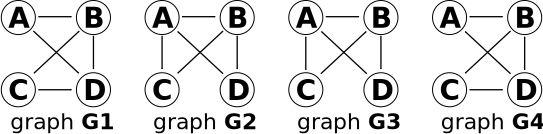
\includegraphics[width=0.6\columnwidth]{q3-graphs.pdf}}

\noindent
There are many ways of defining and storing such graphs.
Below, there are three different examples of such graph definitions, labeled \textbf{D1}, \textbf{D2}, and \textbf{D3}.\\

\noindent
\fbox{%
  \begin{minipage}[t]{0.3\columnwidth}
    definition \textbf{D1}\\
    \emph{adjacency lists}\\[1.1\baselineskip]
    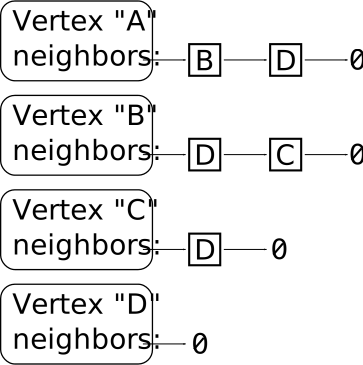
\includegraphics[width=\columnwidth]{q3-adjlist-diagrams.pdf}
  \end{minipage}%
}
\hfill
\fbox{%
  \begin{minipage}[t]{0.3\columnwidth}
    definition \textbf{D2}\\
    \emph{source code}
    \footnotesize
    \verbatimtabinput{Q3.java}
  \end{minipage}%
}
\hfill
\fbox{%
  \begin{minipage}[t]{0.3\columnwidth}
    definition \textbf{D3}\\
    \emph{adjacency matrix}\\[1.1\baselineskip]
    \begin{tabular}{|*{5}{c|}}
      \hline
      \emph{source}
      &
      \multicolumn{4}{l|}{\emph{destination}} \\
        & A & B & C & D \\
      \hline
      A &   & * &   &   \\
      \hline
      B &   &   & * &   \\
      \hline
      C &   &   &   & * \\
      \hline
      D & * & * &   &   \\
      \hline
    \end{tabular}
  \end{minipage}%
}\\

\begin{enumerate}
\item
  For each of the definitions \textbf{D1}, \textbf{D2}, and \textbf{D3}, find out which of the graphs \textbf{G1}, \textbf{G2}, \textbf{G3}, and \textbf{G4} is created or represented.
\item
  One of the graphs is not represented by any of the definitions.
  Which one is it?
  Choose one of the definition styles and use that to describe the graph that was not covered by \textbf{D1}, \textbf{D2}, and \textbf{D3}.
\end{enumerate}

\clearpage

\question

A \emph{spanning tree} is a tree which is embedded in a graph in such a way that
(1) all the vertices of the graph appear in the tree, and
(2) all the edges of the tree are also edges in the graph.
In other words, a spanning tree is composed of all the vertices and some of the edges of the graph.
It is possible to compute a spanning tree by tracing the execution of depth-first search (DFS):
whenever a non-visited vertex is encountered, the edge connecting to it is added to the spanning tree.
This technique also works for breadth-first search (BFS).

\emph{%
For example, assume that you are in the middle of DFS and the current vertex is \textbf{C}.
You would now check whether \textbf{A}, \textbf{B}, or \textbf{F} are already visited.
If now, for example, \textbf{F} is not yet visited, mark the edge connecting \textbf{C} to \textbf{F} as belonging to the spanning tree.}

For a given graph, there usually is more than one spanning tree.
In this question, you are asked to perform DFS and BFS on the graph shown below.
The adjacency matrix is also given, in order to define the iteration order of outgoing edges:
simply read from left to right along the appropriate row of the adjacency matrix.
For example, the order of out-edges from vertex \textbf{C} is: \textbf{A}, \textbf{B}, \textbf{F}.

\begin{center}
  \fbox{%
    \begin{minipage}{0.95\columnwidth}
      \begin{minipage}{0.4\columnwidth}
        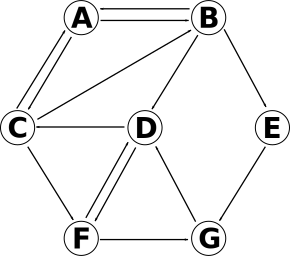
\includegraphics[width=\columnwidth]{q4-graph-diagram.pdf}
      \end{minipage}
      \hfill
      \begin{minipage}{0.45\columnwidth}
        \begin{tabular}{|*{8}{c|}}
          \hline
          \emph{source}
          &
          \multicolumn{7}{l|}{\emph{destination}} \\
            & A & B & C & D & E & F & G \\
          \hline
          A &   & * & * &   &   &   &   \\
          \hline
          B & * &   &   & * & * &   &   \\
          \hline
          C & * & * &   &   &   & * &   \\
          \hline
          D &   &   & * &   &   & * &   \\
          \hline
          E &   &   &   &   &   &   & * \\
          \hline
          F &   &   &   & * &   &   & * \\
          \hline
          G &   &   &   & * &   &   &   \\
          \hline
        \end{tabular}
      \end{minipage}
    \end{minipage}%
  }
\end{center}

\begin{enumerate}
\item
  Perform DFS starting at vertex \textbf{A} and write down the order in which the vertices are visited.
\item
  Perform BFS, also starting at vertex \textbf{A}, and also writing down the visitation order.
\item
  Draw a diagram of the spanning tree rooted at \textbf{A} using depth-first search.
\item
  Draw a diagram of the spanning tree rooted at \textbf{A} using breadth-first search.
\end{enumerate}

\end{document}
